\exercisesetinstructions[Exercises]{ ask a variety of questions dealing with approximating error and sensitivity analysis.}

\exercise{A cylindrical storage tank is to be 2ft tall with a radius of 1ft. Is the volume of the tank more sensitive to changes in the radius or the height?}{The total differential of volume is $\dd V = 4\pi\dd r + \pi\dd h$. The coefficient of $\dd r$ is greater than the coefficient of $\dd h$, so the volume is more sensitive to changes in the radius.}

\exercise{\textbf{Projectile Motion:} The $x$-value of an object moving under the principles of projectile motion is $x(\theta,v_0,t)= (v_0\cos\theta)t$. A particular projectile is fired with an initial velocity of $v_0=250$ft/s and an angle of elevation of $\theta = 60^{\circ}$. It travels a distance of $375$ft in 3 seconds.\bigskip

Is the projectile more sensitive to errors in initial speed or angle of elevation?%
}{Distance of the projectile is a function of two variables (leaving $t=3$): $D(v_0,\theta) = 3v_0\cos\theta$. The total differential of $D$ is $\dd D = 3\cos\theta\dd v_0-3v_0\sin\theta\dd\theta$. The coefficient of $\dd\theta$ has a much greater magnitude than the coefficient of $\dd v_0$, so a small change in the angle of elevation has a much greater effect on distance traveled than a small change in initial velocity.}

\exercise{The length $\ell$ of a long wall is to be approximated. The angle $\theta$, as shown in the diagram (not to scale), is measured to be $85^{\circ}$, and the distance $x$ is measured to be 30'. Assume that the triangle formed is a right triangle.\bigskip

Is the measurement of the length of $\ell$ more sensitive to errors in the measurement of $x$ or in $\theta$?

\begin{minipage}{\linewidth}
\centering
\pdftooltip{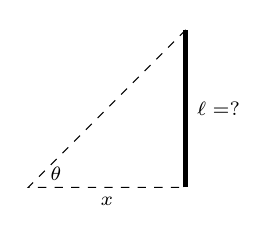
\begin{tikzpicture}
\draw [ultra thick] (1,-1) -- node [pos=.5,right] {\scriptsize $\ell=$?}(1,1);
\draw [dashed] (1,1) -- (-1,-1) node [xshift=10pt,yshift=5pt] {\scriptsize $\theta$} -- node [pos=.5,below] {\scriptsize $x$} (1,-1);
%\draw (-.5,0) -- node [pos=.5,draw=white,fill=white] {\scriptsize $50'$} (1,0);
\end{tikzpicture}}{ALT-TEXT-TO-BE-DETERMINED}
\end{minipage}%
}{Using trigonometry, $\ell = x\tan\theta$, so $\dd\ell = \tan\theta\dd x + x\sec^2\theta\dd\theta$. With $\theta = 85^{\circ}$ and $x=30$, we have $\dd\ell = 11.43\dd x+3949.38\dd\theta$. The measured length of the wall is much more sensitive to errors in $\theta$ than in $x$. While it can be difficult to compare sensitivities between measuring feet and measuring degrees (it is somewhat like ``comparing apples to oranges''), here the coefficients are so different that the result is clear: a small error in degree has a much greater impact than a small error in distance.}

\exercise{It is ``common sense'' that it is far better to measure a long distance with a long measuring tape rather than a short one. A measured distance $D$ can be viewed as the product of the length $\ell$ of a measuring tape times the number $n$ of times it was used. For instance, using a 3' tape 10 times gives a length of 30'. To measure the same distance with a 12' tape, we would use the tape 2.5 times. (I.e., $30=12\times 2.5$.) Thus $D = n\ell$.\bigskip

Suppose each time a measurement is taken with the tape, the recorded distance is within 1/16'' of the actual distance. (I.e., $d\ell = 1/16'' \approx 0.005$ft). Using differentials, show why common sense proves correct in that it is better to use a long tape to measure long distances.%
}{With $D = n\ell$, the total differential is $\dd D = \ell\dd n+ n\dd\ell.$ If one measures with a short tape, $n$ must be large and hence $n\dd\ell$ is going to be greater than when a large tape is used (wherein $n$ will be small).}

\exercisesetend
